\documentclass{article}
\usepackage{multirow}
\usepackage{hyperref}
\usepackage{graphicx}
\usepackage{xcolor}
\usepackage{float}

\title{Root Digger: a root placement program for phylogenetic trees}
\author{Ben Bettisworth, Alexandros Stamatakis}
\date{\today}

\newcommand{\RootDigger}{RootDigger}
\newcommand{\RootDiggertt}{\texttt{RootDigger}}
\newcommand{\BenComment}[1]{{\bf \color{blue} {#1}}}
\newcommand{\AlexisComment}[1]{{\bf \color{green} {#1}}}

\begin{document}
\begin{abstract}
  In phylogenetic analysis, it is common to infer trees which are unrooted. This
  is to say, it is unknown which node is the most recent common ancestor of all
  the taxa present in the phylogenetic tree. This information is often desirable,
  as it provides a direction to the edges in the tree. There exist several
  methods to recover a root, including midpoint rooting and using a special taxon
  as a so called outgroup. Additionally, a non-reversable Markov model can be used
  to compute the likelihood of a root. In this paper, we present software which
  uses a provided non-reversable model to compute the most likely root location.
\end{abstract}

\maketitle

% Main Points:
% - Rerunning analysis with outgroups is expensive, and can introduce errors
% - Midpoint rooting is a joke
% - This is fast and accurate.


\section{Introduction}

% Outline:
% - What is rooting
% - Why do we need it
% - Existing methods
% - What this method is
% - Why should we use this method

When inferring phylogenetic trees, many phyogenetic inference tools
\cite{stamatakis_raxml_2014} \cite{nguyen_iq-tree:_2015} will infer an unrooted
tree. This due to a common (and default) assumption: reversibility of the
character substituion process \cite{felsenstein_evolutionary_1981}. This
assumption makes the problem of infering a phylogentic tree much more tractable,
but by making this assumption the ability to distinguish a root is lost. A
rooted phylogenetic tree is desirable, though, as it can resolve long standing
disputes regarding the placment of large clades on the tree of life
\cite{dunn_animal_2014} for example.

There are several methods to recover the root on an existing phylogenetic tree,
which generally fall into one of three categories: methods which use additional
topological information not present in the molecular data; methods which utilize
some variation of the molecular clock hypothesis; and methods which use a
non-reversable model.

Methods that use additional topological information take advantage of prior
knowledge about the world, which isn't present in the data that is used to infer
a tree. In particular, knowledge about species which are distantly related can
be used to add a so-called outgroup to phylogenetic analysis. This outgroup can
then be used to place the root on the tree, as the most recent common anscestor
of the ingroup and the outgroup must be the root of the tree.

There are challenges to adding an outgroup to an analysis. Gatsey et.al.
\cite{gatesy_how_2007} \BenComment{How do I cite papers directly, should I just
  use the number?} showed how adding a single taxa to an analysis can
significantly impact the resulting tree topology, even for the taxa which were
already present in the analysis (the ingroup). Holland
\cite{holland_outgroup_2003} investigates this phenomenon in simulations, and
finds that outgroups effecting the topology of ingroups can be uncomfortably
common.

Alternativly, molecular clock analysis can be used to place a root without prior
topological knowledge\cite{yang_computational_2006}. The molecular clock
hypothesis says that base substitution "ticks" at stochastically constant rate.
Using this assumption, or some variant, a likely root can be placed on the root.
A simple version of this analysis is midpoint rooting, which uses a constant and
static molecular clock assumption.

Molecular clock analysis has its own difficulties. In particular, the clock
does not "tick" at a constant rate all over the tree as shown in
\cite{steiper_primate_2006} and \cite{li_molecular_1987}. Relaxed clock models
exist which can help with this problem, but are not always successful as shown
in \cite{battistuzzi_performance_2010}.

The final method that can place a root on a tree is to perform the phylogenetic
analysis using a non-reversable model. By using a non-reversable model, we can
place a direction of time for the branches on a tree
\cite{yap_rooting_2005}. Several software packages are able to infer a
phylogenetic tree under an unreversable model, thereby inferring a root
\cite{nguyen_iq-tree:_2015} \cite{ronquist_mrbayes_2003}.

Non-reversible models for phylogenetic trees come in many forms. For example,
accounting for duplication, transfer and loss events yields a non-reversible
model. In particular, duplication events has been used to root a tree
\cite{emms_stride:_2017}.

A natural alternative to produce a non-reversible model is to drop the
reversibility assumption of the standard phylogenetic inference models.
Unfortunately, dropping this assumption can significantly effect the time
required to find a good (high likelihood) phylogenetic tree. As a workaround, an
unrooted tree which has already been inferred can be evaluated for possible root
locations under a non-reversible model. With this method, we can find the most
likely root. To this end, we introduce a phylogenetic tool called \RootDiggertt,
which performs this analysis.

%In phylogenetic analysis, it is common to infer an unrooted tree. This is due to
%several factors, including: speed of analysis
%\cite{felsenstein_evolutionary_1981}, tool support \cite{stamatakis_raxml_2014},
%and availability of other methods \cite{huelsenbeck_inferring_2002}. Instead,
%root placement analysis has generally been performed using additional data, such
%as outgroups, or via a molecular clock hypothesis. 
%
%% reasons outgrouping sucks:
%% - additional computational requirements
%% - selecting an outgroup is error prone
%% - outgroup can effect the topology of the ingroup
%
%Outgrouping is a rooting technique that involves adding additional data beyond
%the taxa in question for the phylogeny. Unfortunately, including an outgroup in
%the dataset introduces both increased computational load, as well as systematic
%errors \cite{gatesy_how_2007} \cite{holland_outgroup_2003}. Particularly
%relevant errors are changes to the ingroup topology when an outgroup is added.

\section{Methods}

Phylogenetic inference requires a model of evolution. Commonly, a Markov
substution process is used \cite{yang_computational_2006}, along with sequence
data such as DNA sequences.  Using this model of evolution, a probability of one
species evolving into another in a specified amount of time can be calculated as
the probability of one sequence evolving into another. By representing each edge
of the tree as one of these Markov processes, we can calculate the likelihood of
both the subsutution processes, and the choosen topology of the tree.

Since it is commonly assumed that the Markovian process is reversible, the tree
that results from this process lacks a root. When we relax the reversibility
assumption, then we also loose the benefits of the pulley principle
\cite{felsenstein_evolutionary_1981}. Since the root location effects the
likelihood of the tree, then multiple rootings need to be attempted for each
tree in order to find the highest likelihood.  In the worst case, this increases
the work {\em per tree} by a factor of $\mathcal{O}(n)$. While there are methods
to reduce the amount of work required, eliminating the reversibility assumption
drastically increases the effort required to infer a tree.

Instead attempting to find the root for every tree encountered during the tree
search, we can instead infer an unrooted tree using a reversible model, and then
infer the root with a reversible model, using an exhaustive search.
This is faster, as it skips the expensive step of looking for good rootings
during intermediate trees. There are still additional challenges though, as the
likelihood function for rooting on a phylogenetic tree is filled with local
maxima \cite{huelsenbeck_inferring_2002}.

\RootDiggertt{} has two modes, search and exhaustive. In search mode,
the program starts by selecting a set of branches at random (with
replacement).  The set of random branches will be used as the initial root
location for the next stages of the search. The search then proceeds by setting
the initial model parameters to be uniform, and then:

\begin{enumerate}
  \item Optimize Rates (via BFGS).
  \item Optimize Frequencies (via BFGS).
  \item Find and move to the next best root (via Recursive Brent's Method).
  \item Check stopping criterion:
        \begin{itemize}
          \item (In early stop mode) Is the current root location the same as
                the last iteration's root, taking into account branch lengths?
          \item Is the difference between the current log likelihood to previous
                log likelihood less than some tolerance?
        \end{itemize}
  \item If a stopping criterion is met: stop; otherwise repeat from 1 for a
        maximum of 1000 iterations.
\end{enumerate}

Step 3 is performed by first calculating the top 5\% of root locations at the
midpoint by likelihood. We use this top 5\% to conduct a more detailed search
along the branch for the optimal root location. To do this search, we view the
problem as finding the maximum argument for some function $f_i(\alpha)$ which
calculates the likelihood of the tree with a root position $\alpha t_i$ along
the branch $i$, where $0 \leq \alpha \leq 1$. Therefore, we are looking for $i$
and $\alpha$, which will indicate which branch and where on that branch to place
the root.

By viewing the problem in this way, the problem can be solved using more
efficient 1 dimensional optimization techniques, which involve finding the root
of the derivative. In this case, we use Brent's method, due to the lack of
access to a second derivative \footnotemark.

\footnotetext{We could compute a derivative, but the library that we use
  computes logged likelihoods, and we require them unlogged. The effort to rewrite
  the functions that would compute this derivative was deemed to be too much
  relative to the savings. In principle, the computation could be done.}

A limitation of root finding methods is that they will fail to find {\it all} the
roots of a function if there are multiple roots. To compensate, we need to
search for bracketing windows that can be used to safely find roots.
Unfortunately, we are not aware of a general method for finding such bracketing
windows, so a recursive method is employed, were the search range is reduced in
half and searched for appropriate \footnotemark windows.

\footnotetext{Appropriate here means that the sign of the function in question has
  opposite signs at the endpoints of the window.}

In exhaustive mode, \RootDiggertt{} performs the same steps with two
differences: every root is tried, not just a subset; and the root location is
limited to the current branch. This has the effect of finding the best
likelihood that a root is placed along this branch. The best root location for
each branch, and a likelihood weight ratio is reported
\cite{strimmer_inferring_2002}.

\section{The Software}

In order to implement both phylogenetic inference and non-reverable models,
\RootDigger has two major dependancies: GNU Scientific Library (GSL)
\cite{gough_gnu_2009} and the Phylogenetic Likelihood Library (LibPLL)
\cite{flouri_phylogenetic_2015}. GSL is used to assist in the decomposition of a
non-symmetric rate matrix, and LibPLL is used for efficient likelihood
calculation.

Usage of \RootDigger is simple. All that is required is a metric tree in newick
format, and an alignment in either phylip or fasta format. The code,
documentation, experiment scripts, datasets, as well as any modifications to existing
libraries can be found at
github\footnote{\url{https://github.com/computations/root_digger}}.

\section{Experiments and Results}


To validate \RootDiggertt{}, we conducted several experiments on both simulated
data and emperical data. Furthermore, we also used Likelihood Weight Ratios
(LWR) \cite{strimmer_inferring_2002} to asses the confidence in a root
placement. Finally, we investigated how model selection effects the placement
and confidence in a particular root placement.

\subsection{Simulations}

We first investigated using simulated data using a pipeline, which was to test
against simulated data, and compare to IQ-TREE \cite{nguyen_iq-tree:_2015}. The
pipeline is:

\begin{enumerate}
  \item Generate a random tree with ETE3 \cite{huerta-cepas_ete_2016} and random
        model parameters.
  \item Simulate an MSA with indelible \cite{fletcher_indelible:_2009}
  \item Run RootDigger and IQ-TREE \cite{nguyen_iq-tree:_2015} on the simulated MSA, given the generated random tree.
  \item Compute comparisons
        \begin{enumerate}
          \item Calculate rooted RF distance with ETE3 \cite{robinson_comparison_1981}
          \item Map root placement onto original tree.
        \end{enumerate}
\end{enumerate}

Additionally, we repeat the pipeline for a specified number of iterations in
order to determine how much the initial seed matters. Furthermore, we vary two
additional parameters parameters: sites and taxa. The results from these
experiments are summarized in table \ref{table:results}. The distance given is
the average distance from the branch with the true root to the inferred root
location over 100 trials. In addition to the simulated pipeline, we validated
root digger with empirical data. The empirical datasets used are listed in
table~\ref{table:datasets}.  These experiments were timed, and the results can
be found in table \ref{table:time_results}

\begin{table}
  \begin{center}
    \begin{tabular} { l c c c}
   & \multicolumn{3}{c} {Taxa}\\
   Sites & 10 & 50 & 100 \\
   \hline
   1000   & 2.758 & 5.918 & 7.302 \\
   4000   & 2.818 & 5.972 & 7.322 \\
   8000   & 2.800 & 5.898 & 7.184 \\
\end{tabular}
\caption{Table of results. Numbers are topological distance from the branch with
the true root to the inferred root.}

    \label{table:results}
  \end{center}
\end{table}

\begin{table}
  \begin{center}
    \begin{tabular} {l c c c c c c}
   & \multicolumn{6}{c} {Taxa}\\
   Sites & \multicolumn{2}{c}{10} & \multicolumn{2}{c}{50} &
   \multicolumn{2}{c}{100} \\
        & RD & IQ & RD & IQ& RD & IQ\\
   1000 & DUMMY & DUMMY & DUMMY & DUMMY & DUMMY & DUMMY \\
   4000 & DUMMY & DUMMY & DUMMY & DUMMY & DUMMY & DUMMY \\
   8000 & DUMMY & DUMMY & DUMMY & DUMMY & DUMMY & DUMMY \\
\end{tabular}
\caption{Table of execution times for Root Digger and IQ-TREE}

    \label{table:time_results}
  \end{center}
\end{table}


\subsection{Empirical Data}

The empirical datasets were chosen to have an existing, strongly supported
outgroup. The experiments were run on datasets with the outgroup included, as
well as with the outgroup removed.

\begin{table}[H]
  \begin{center}
    \begin{tabular} { l c c c}
   Dataset & \#Taxa & \#Sites & Source \\
   \hline
   AngiospermsCDS12 & 35 & 864029 & \cite{ran_phylogenomics_2018}\\
   AngiospermsCDS & 35 & 1296043 & \cite{ran_phylogenomics_2018}\\
   Grasses & 245 & 4973 & \cite{christin_molecular_2014}\\
   Ficus & 200 & 5552 & \cite{cruaud_extreme_2012}\\
   SpidersMissingSpecies & 33 & 1097842 & \cite{leduc-robert_phylogeny_2018}\\
   SpidersMitocondrial & 34 & 12479 & \cite {leduc-robert_phylogeny_2018}\\
\end{tabular}
\caption{Table of emperical datasets used for validation}

    \label{table:datasets}
  \end{center}
\end{table}

\begin{table}
  \begin{center}
    \begin{tabular} { l || c c  || c c  || c c || }
   Dataset & \multicolumn{2}{c ||}{Distance} & \multicolumn{2}{c ||}{Path Distance} &
   \multicolumn{2}{c ||}{Time} \\
           & RD & IQ & RD & IQ & RD & IQ \\
   \hline
   AngiospermsCDS12       & &  & & & &\\
   AngiospermsCDS         & &  & & & &\\
   Grasses                & &  & & & &\\
   Ficus                  & &  & & & &\\
   SpidersMissingSpecies  & &  & & & &\\
   SpidersMitocondrial    & &  & & & &\\
\end{tabular}
\caption{Results for empirical datasets. Distance is the distance from the
estimated root placement to the true root placement, taking into account branch
lengths. Path Distance is the topological distance from the estimated root
placement to the true root placement. RD Time and IQ time are the run times}

    \label{table:emperical_results}
  \end{center}
\end{table}

\subsection{Likelihood weight ratios}

Additional experiments were conducted to investigate the nature of the
distribution of root placements. To do this, we ran \RootDiggertt{} on the empirical
datasets listed in table \ref{table:datasets} in exhaustive mode without early
stop. This mode calculates a likelihood weight ratio for a root placement on
each branch, and reports it.

\begin{figure}
  \begin{center}
    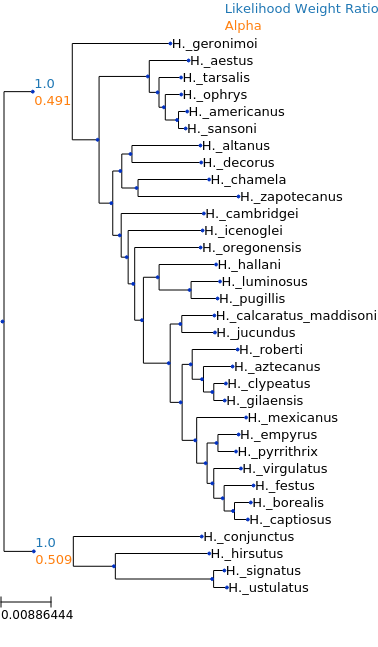
\includegraphics[width=.75\linewidth]{figs/spiders/missing_species_no_outgroup_lwr.png}
    \caption{SpidersMissingSpecies dataset analyzed without an outgroup.}
    \label{fig:spiders-missing-species-no-outgroup}
  \end{center}
\end{figure}

\begin{figure}
  \begin{center}
    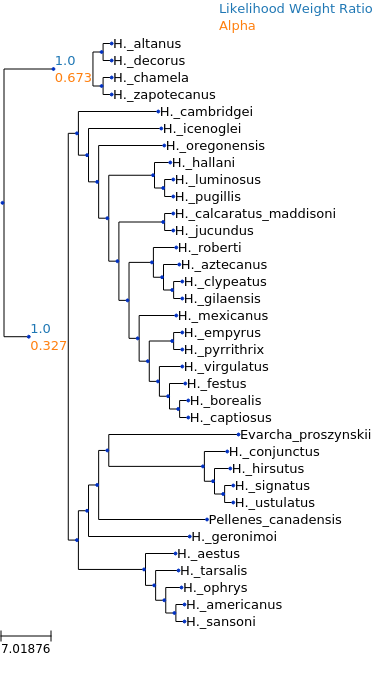
\includegraphics[width=.75\linewidth]{figs/spiders/missing_species_outgroup_lwr.png}
    \caption{SpidersMissingSpecies dataset analyzed with an outgroup.}
    \label{fig:spiders-missing-species-outgroup}
  \end{center}
\end{figure}

\begin{figure}
  \begin{center}
    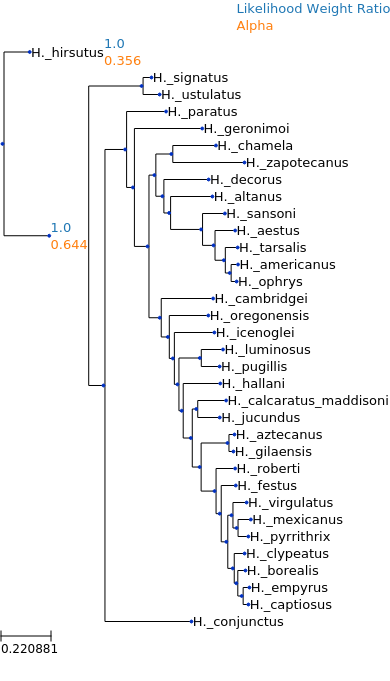
\includegraphics[width=.75\linewidth]{figs/spiders/mito_no_outgroup_lwr.png}
    \caption{SpidersMitocondrial dataset analyzed without an outgroup.}
    \label{fig:spiders-mito-no-outgroup}
  \end{center}
\end{figure}

\begin{figure}
  \begin{center}
    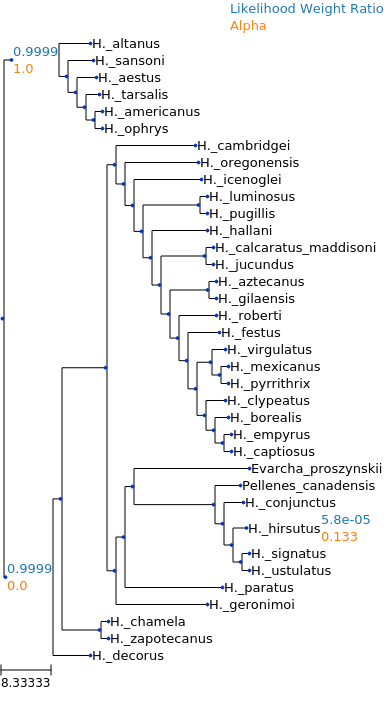
\includegraphics[width=.75\linewidth]{figs/spiders/mito_outgroup_lwr.png}
    \caption{SpidersMitocondrial dataset analyzed with an outgroup.}
    \label{fig:spiders-mito-outgroup}
  \end{center}
\end{figure}

%\begin{figure}[H]
%  \begin{center}
%    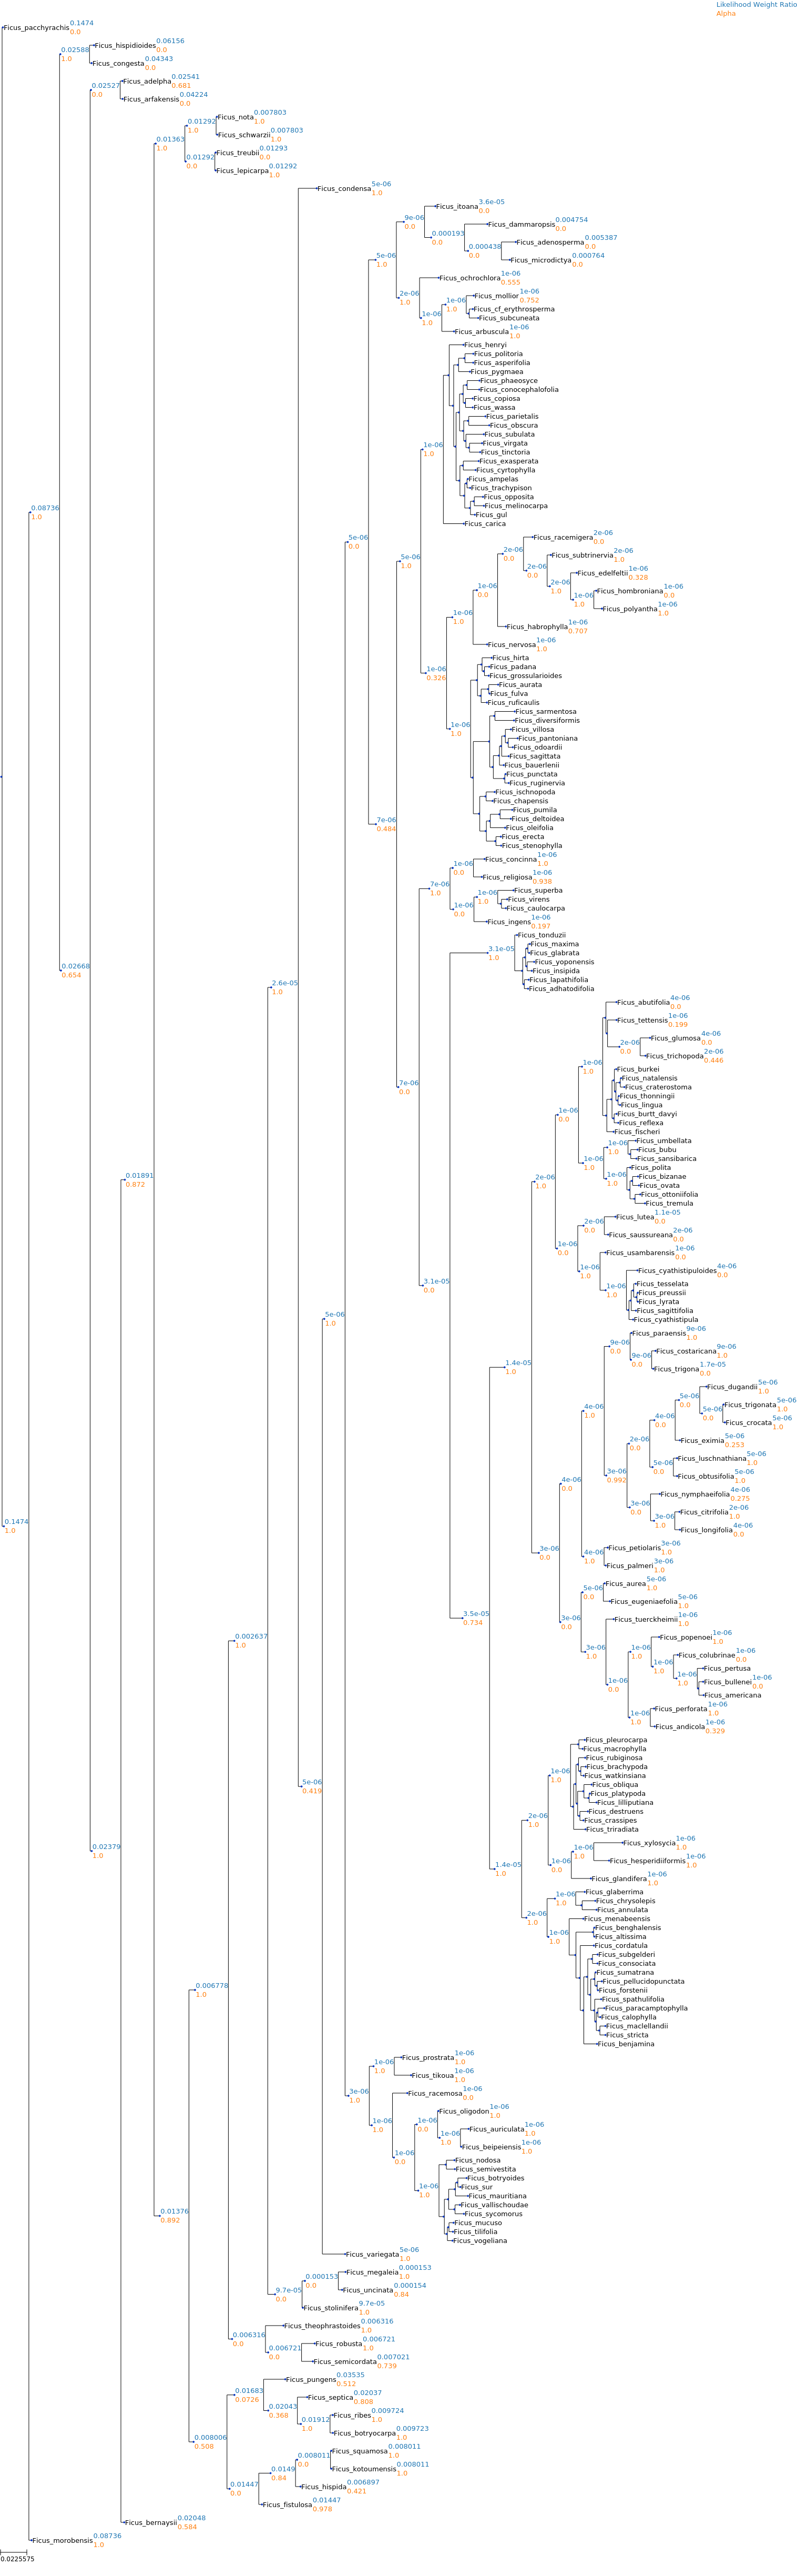
\includegraphics[width=.75\linewidth]{figs/ficus/ficus_no_outgroup_lwr.png}
%    \caption{Ficus dataset analyzed without an outgroup.}
%    \label{fig:ficus-no-outgroup}
%  \end{center}
%\end{figure}
%
%\begin{figure}[H]
%  \begin{center}
%    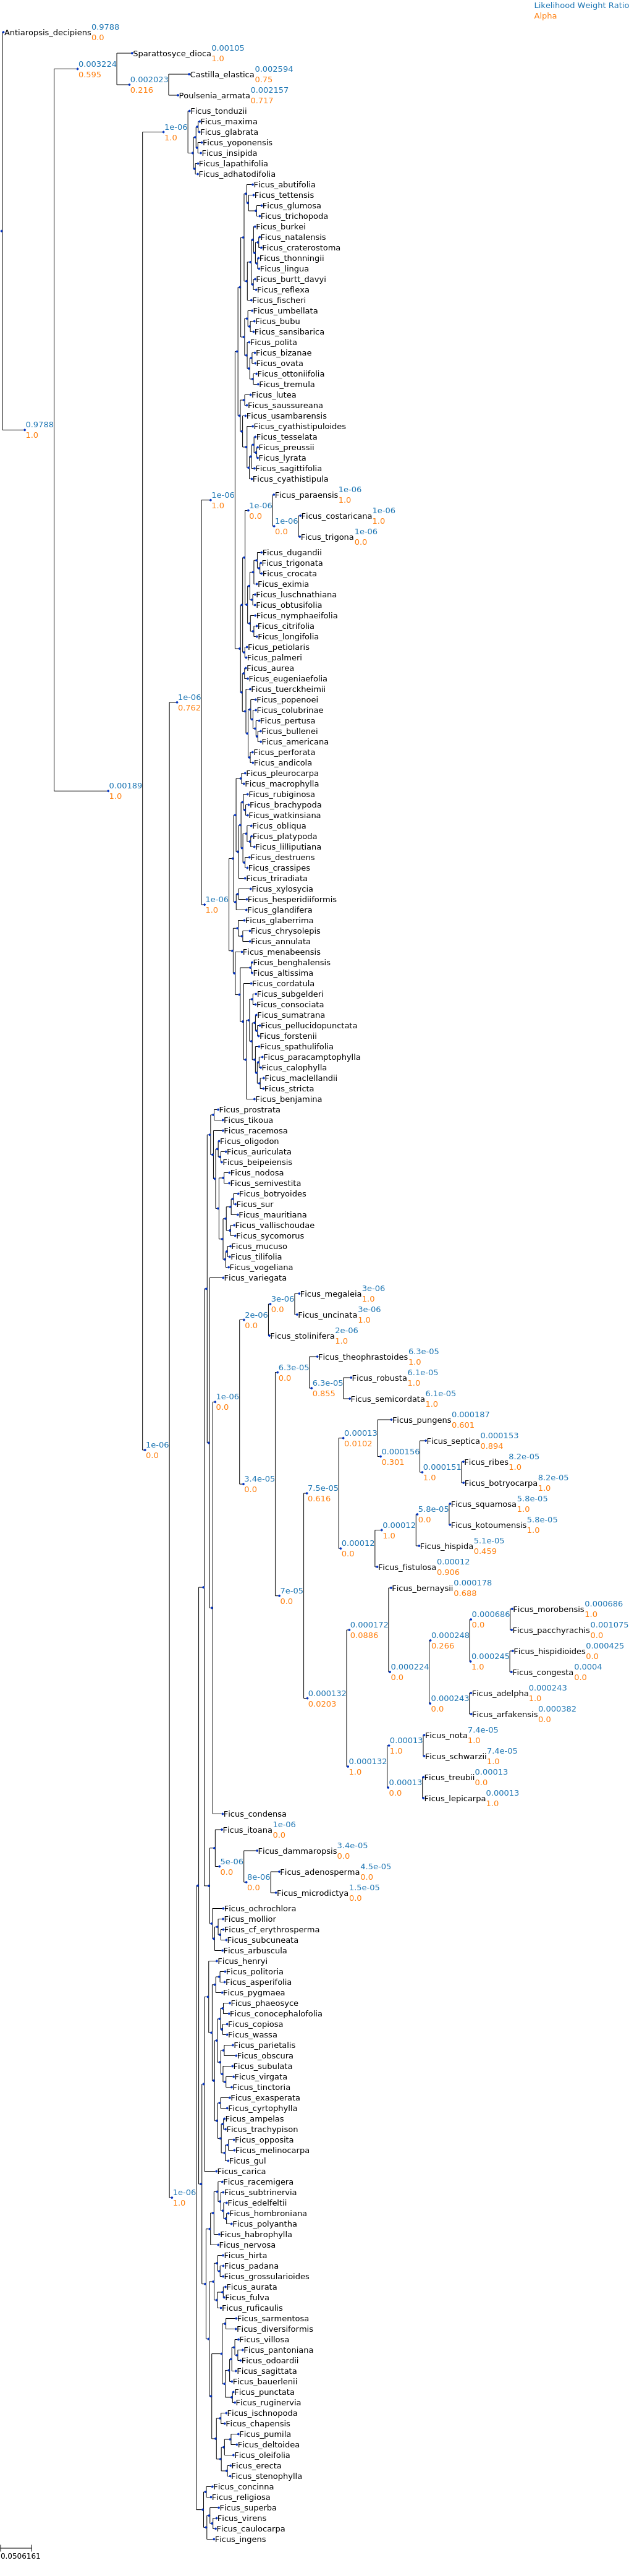
\includegraphics[width=.75\linewidth]{figs/ficus/ficus_outgroup_lwr.png}
%    \caption{Ficus dataset analyzed with an outgroup.}
%    \label{fig:ficus-outgroup}
%  \end{center}
%\end{figure}

\begin{figure}
  \begin{center}
    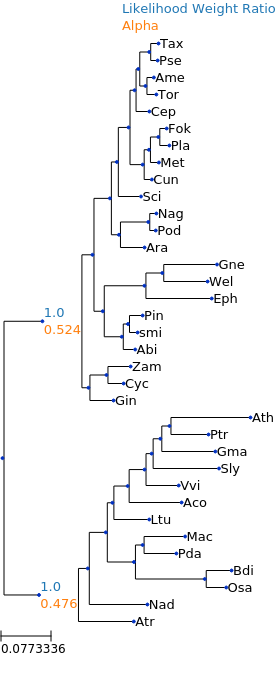
\includegraphics[width=.5\linewidth]{figs/angio/cds12_no_outgroup_lwr.png}
    \caption{AngiospermsCDS12 dataset analyzed without an outgroup.}
    \label{fig:angio-cds12-no-outgroup}
  \end{center}
\end{figure}

\begin{figure}
  \begin{center}
    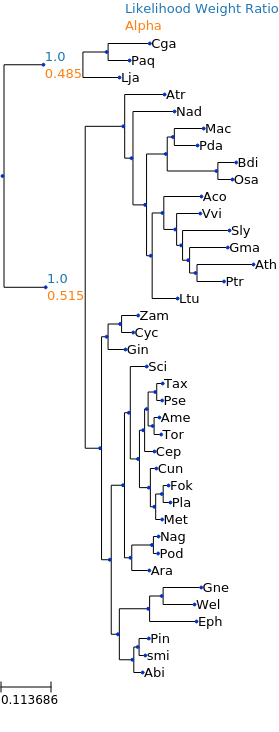
\includegraphics[width=.5\linewidth]{figs/angio/cds12_outgroup_lwr.png}
    \caption{AngiospermsCDS12 dataset analyzed with an outgroup.}
    \label{fig:angio-cds12-outgroup}
  \end{center}
\end{figure}

\subsection{Effect of model selection on results}

We also investigated the effect of model selection on the results. We did this
by running \RootDiggertt{} in exhaustive mode with a varying number of rate
categories for the SpidersMitocondrial dataset. The result of this analysis can
be seen in figures~\ref{fig:spiders1rate} and \ref{fig:spiders2rate}. Of
particular note is that increasing the number of rate categories not only
moves the root to an erroneous location, it increases the confidence
significantly.

\begin{figure}[H]
  \begin{center}
    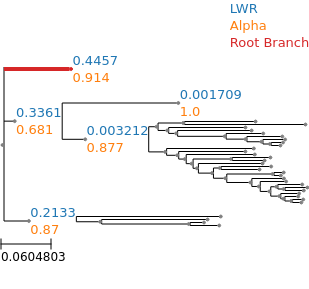
\includegraphics[width=.75\linewidth]{figs/spiders/1rate.png}
    \caption{SpidersMitocondrial dataset analyzed with 1 rate category.}
    \label{fig:spiders1rate}
  \end{center}
\end{figure}

\begin{figure}
  \begin{center}
    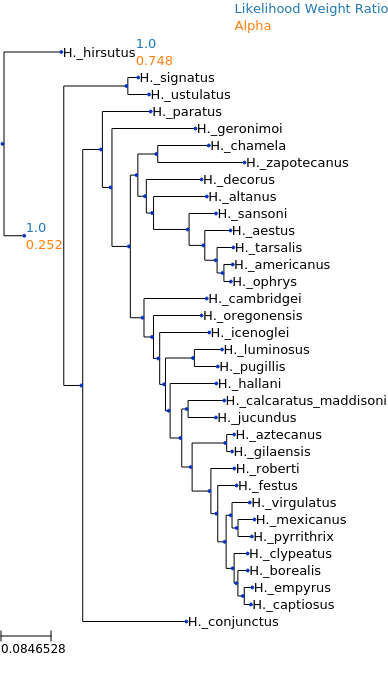
\includegraphics[width=.75\linewidth]{figs/spiders/2rate.png}
    \caption{SpidersMitocondrial dataset analyzed with 2 rate categories.}
    \label{fig:spiders2rate}
  \end{center}
\end{figure}

\section{Discussion}

\section{Conclusion}

\bibliographystyle{acm}
\bibliography{main}

\end{document}
